\chapter{Architecture}

\section{System Context}
We have a single \emph{JassTracker} system without any external services.

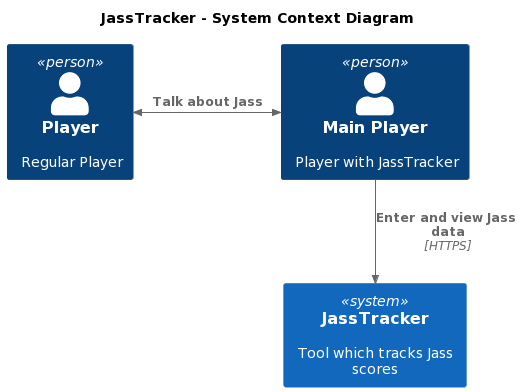
\includegraphics[width=\textwidth]{resources/diagrams/c4-1-system-context}

\section{Container}
Our system is split into three containers.
Each container uses its own technology and could be (relatively) easily exchanged.

The \emph{Frontend} is our single-page-application which provides the user interface.
We decided to use a dedicated SPA instead of server rendered pages to improve the user experience.
When a user enters a score, only a small fraction of the whole page needs to be updated.

The \emph{Backend} provides a REST-API-Endpoint which will be used by the \emph{Frontend}.
All business logic will be implemented and tested here, providing pre-processed and easy to digest data upon request.
Having a public REST-API enforces a clean separation and makes testing early on easier.

The \emph{Database} is a simple PostgreSQL database used to store our data.

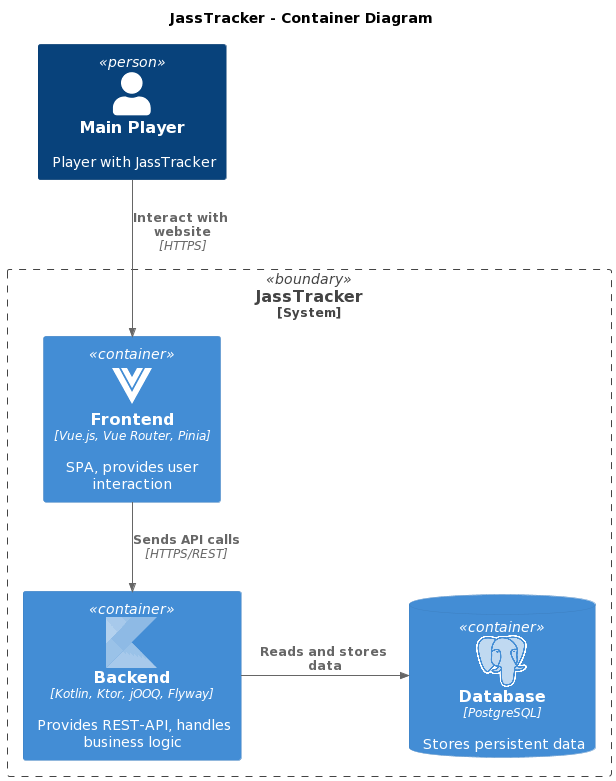
\includegraphics[width=\textwidth]{resources/diagrams/c4-2-container}

\section{Components}

\subsection{Frontend}
The frontend is a single-page-application with a focus on component driven design.
Basically everything is a component, which providers us with high flexibility.
Code can easily be reused and separated from the view files, which themselves stay clean.
The data is received from the Backend via REST API calls in different services that that then provide the data to the according models/views.

\subsection{Backend}
The backend is structured into layers, following the clean-architecture principle.
This means that the \emph{Domain} is in the center, being responsible for all business logic.
Technology-dependent logic is extracted to an outer layer, ensuring they could be easily changed in the future.
We have three technology-specific components:
\begin{itemize}
    \item \emph{Web API}, responsible for the REST-API (Routing, Authentication)
    \item \emph{Data Access}, responsible for connecting to and migrating the database
    \item \emph{Bootstrap}, responsible for application startup and configuration management
\end{itemize}

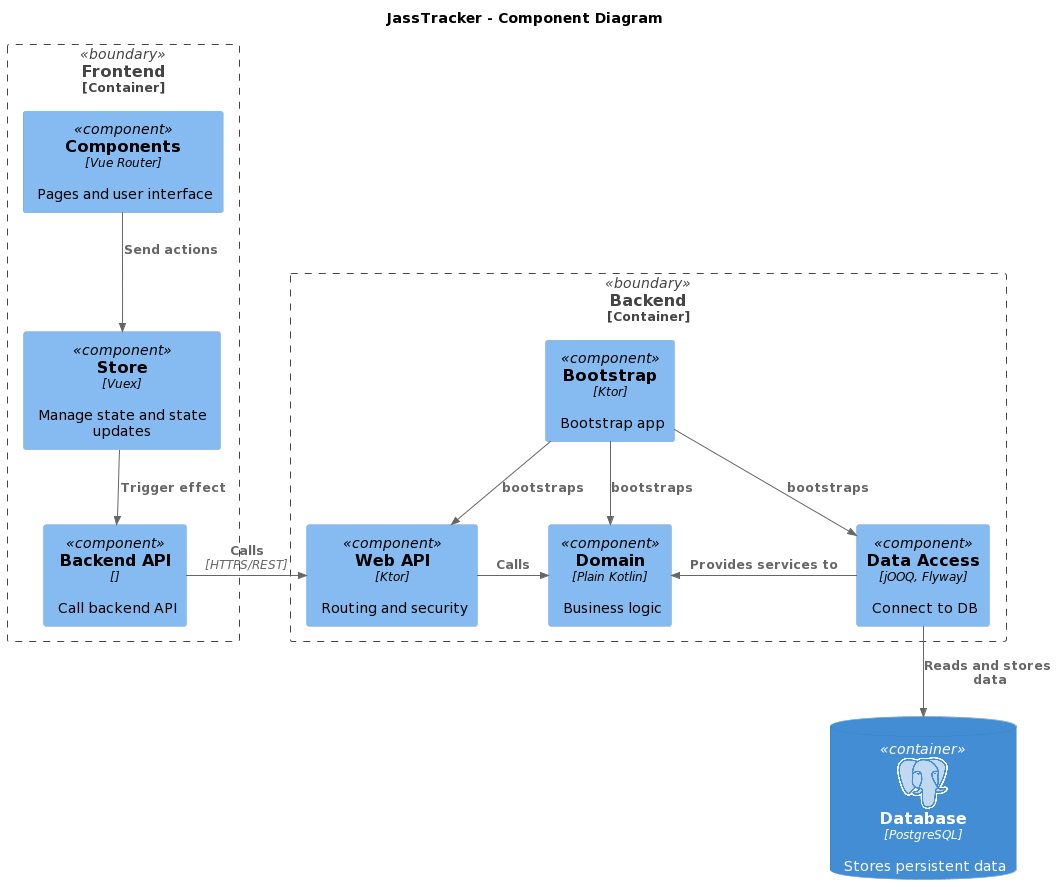
\includegraphics[width=\textwidth]{resources/diagrams/c4-3-component}

\section{Deployment Overview}
\label{sec:architecture_deployment}
Our deployment architecture strives for maximum simplicity while remaining flexible and extensible.
To achieve that goal, a few decisions were made:
\begin{itemize}
    \item use a single host to keep it simple
    \item use docker to make deployments portable
    \item use a reverse proxy to enable a separate staging environment
    \item use one database container for all environments to preserve resources
\end{itemize}

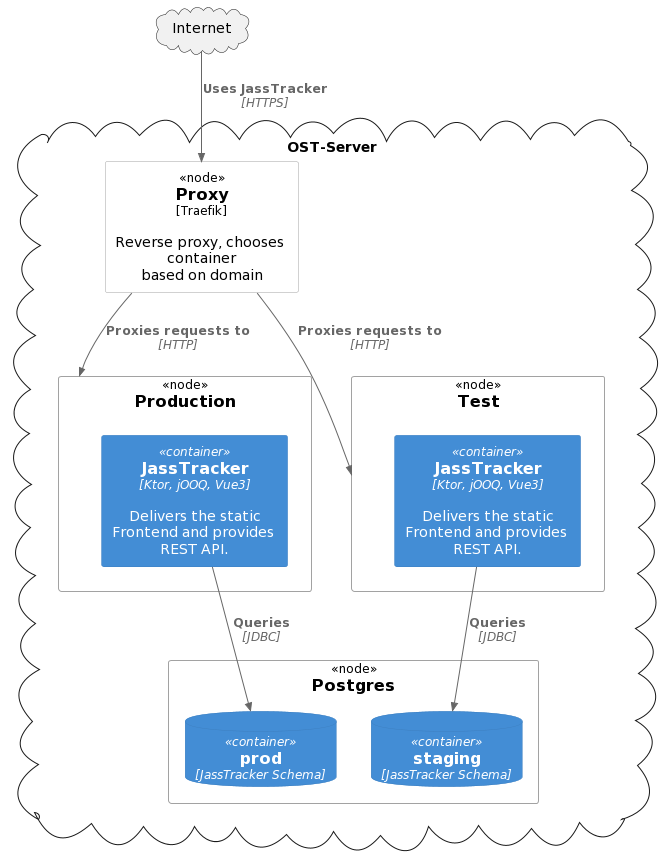
\includegraphics[width=\textwidth]{resources/diagrams/c4-deployment}
